\chapter{Case Study: Strain and Acceleration of Cantilevered Beam} \label{c:accel}

In Chapter~\ref{c:strain} we examined the data acquisition system for measuring the static response of a cantilevered beam using a single strain gage.  In this chapter we'll consider adding an accelerometer to the tip of the beam to simultaneously measure the strain (at the root) and the acceleration (at the free-end) of the beam.  The DAQ system is illustrated in Figure~\ref{f:strainampdaq}.

\begin{figure}[hbt!]
\centering
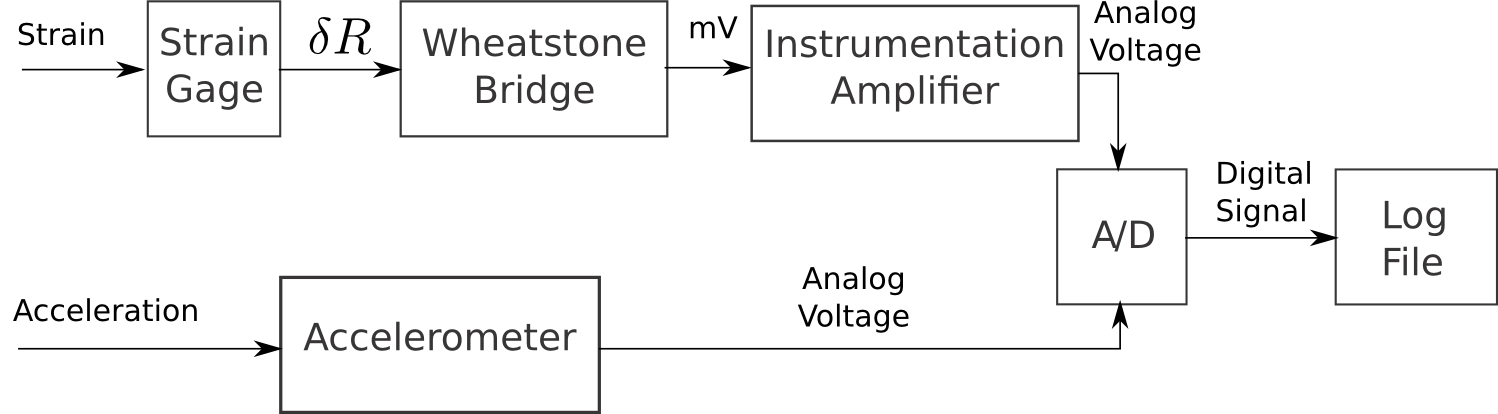
\includegraphics[width=\FigWidth\textwidth]{strain_amp_daq.png}
\caption{A data acquisition including strain gage and accelerometer.}
\label{f:strainampdaq}
\end{figure}

\section{Amplifying the Strain Signal}
Hopefully in Chapter~\ref{c:strain} you discovered that the output of a strain gage (with a Wheatstone bridge) is a small voltage---typically just a few millivolts.  This is a bit of a problem because a typical A/D operates with much larger input range: e.g., $\pm \unit[1.0]{V}$ or $\pm \unit[10.0]{V}$.  As we discussed in Chapter~\ref{c:daq}, the resolution of an A/D is finite, so using an A/D with a range much larger than the anticipate analog voltage input will have poor performance.

To improve the situation we can add an amplifier---the \emph{instrumentation amplifier} shown in Figure~\ref{f:strainampdaq}.  The gain of the amplifier ($K$) is constant multiplier so that the output voltage ($V_o$) is the product of the input voltage ($V_i$) and the gain, i.e.,
\[ V_o = K (V_i). \]

\begin{ex}
Ideally we would choose the gain of our amplifier such that the maximum anticipated voltage will be equivalent to the full-scale range setting of our A/D.  Consider the following strain gage scenario:
\begin{itemize}
\item Strain gage factor: $GF=2.0$
\item Wheatstone bridge excitation voltage: $V_s=\unit[9.0]{V}$
\item Maximum anticipated strain: $\epsilon=\unitfrac[0.001]{m}{m}$
\item A/D range: $E_{FSR}=\pm \unit[1.0]{V}$
\end{itemize}
What would be an appropriate gain setting for an amplifier that we would use in the DAQ system shown in Figure~\ref{f:strainampdaq}?
\end{ex}

\ifsolutions
\begin{soln}
First we need to predict the maximum voltage that we might anticipate from the Wheatstone bridge.  Using (\ref{e:gagebridge}
\[
V_o \approx V_s\left( \frac{(\mathrm{GF})\epsilon}{4} \right).
\]
and the parameters in the exercise we can anticipate the the maximum voltage output $V_o \unit[4.5]{mV}$.  We would like to amplifiy this so that the output of the amplifier is equivalent to the full scale range (\unit[1]{V}).  A gain of 222.2 would give us exactly \unit[1]{V} of maximum output.
\end{soln}
\fi

\section{Accelerometer}
Unsurprisingly an accelerometer is a device for measuring acceleration.  Below are exercises to explore the application of a particular accelerometer to measuring the free response of a cantilevered beam.

\begin{ex}
Look-up the datasheet for the Analog Devices ADXL 335 accelerometer.  (The datasheet can be found online and is also available on the course website.)
\begin{itemize}
\item Read the section ``Theory of Operation''.  Write a few (1--2) sentences to summarize how the device measures acceleration.
\item Assuming a supply voltage of \unit[3]{V}...
  \begin{itemize}
  \item What is the maximum measurable acceleration: in g's and in \unit[]{m}{s$^2$}?
  \item What is the sensitivity of the accelerometer (with appropriate units)?
  \item (Hint: these quantities are listed in the ``Specifications'' section.)
  \end{itemize}
\end{itemize}
\end{ex}

\ifsolutions
\begin{soln}

\end{soln}
\fi



\begin{ex}
Given the cantilevered beam properties described in Exercise~\ref{ex:beamvib} and the free response of the model given in (\ref{e:damped}),
\begin{itemize}
\item What is the maximum acceleration at the free-end of the beam  you might anticipate for the free response of the system with the following initial conditions: $y(0)=\unit[10]{cm}$ and $\dot{y}(0)=0$? (Hint: you will need to differentiate the expression (\ref{e:secondfree}) and you can assume $\zeta=0$ and $\phi=0$. Check your units!)
\item Given this maximum acceleration and the sensitivity of the ADXL 335 from the previous exercise, what is the maximum voltage you should expect as output from an ADXL 335 mounted at the free-end of the beam?
\end{itemize}
\end{ex}

\ifsolutions
\begin{soln}
We need to differentiate twice the expression from (\ref{e:secondfree}) with $\zeta=0$ and $\phi=0$.  
\[
y(t) = C \left( \cos(\omega_n t ) \right)
\]
Using (\ref{e:C}) to evaluate the constant $C$ with these conditions we find that $C=y_o$, so...
\begin{eqnarray}
y(t) & = & y_o \left( \cos(\omega_n t ) \right) \\
\dot{y}(t) & = & y_o * \omega_n \left(-\sin(\omega_n t ) \right) \\
\ddot{y}(t) & = & y_o * \omega_n^2 \left( -\cos(\omega_n t ) \right) \\
\ddot{y}(t) & = & \unit[10]{cm} (\unitfrac[32.6]{rad}{s})^2 \left( -\cos(\omega_n t ) \right) \\
\ddot{y}(t) & = & \unit[10]{cm} (\unitfrac[32.6]{rad}{s})^2 \left( -\cos(\omega_n t ) \right) \\
\ddot{y}(t) & = & \unitfrac[106]{m}{s^2} \left( -\cos(\omega_n t ) \right) \\
\ddot{y}(t) & = & \unit[10.8]{g} \left( -\cos(\omega_n t ) \right) 
\end{eqnarray}
So the amplitude of the acceleration is \unit[10.8]{g}.  The sensitivity of the ADXL 335 is \unit[300]{mV}{g} which indicates that the maximum output from the accelerometer is $10.8*300 = \unit[3240]{mV} = \unit[3.24]{V}$. However, the maximum acceleration the device can sense is $\pm\unit[3]{g}$, so we should probably start with an initial displacement of less than \unit[10]{cm}!
\end{soln}
\fi


